\subsection{Objetivo}
Conocer e implementar una técnica de localización utilizada en aplicaciones reales, específicamente para los robots \textit{Rhino} y \textit{Minerva} en los museos \textit{Deutsches Museum Bonn} y \textit{National Museum of American History}, respectivamente \parencite{Dieter1999}. Se utilizará Processing como herramienta de visualización de la técnica de localización.

\subsection{Introducci\'on}

\quotes{La localización robótica ha sido considerado como uno de los problemas fundamentales de la robótica. El objetivo de la localización es lograr estimar la posición del robot en un ambiente, apoyándose en un mapa de éste y con lecturas de sensores} \parencite{Dieter1999}. Tomando como base esta publicación de Dieter Fox, et. al. conoceremos los tipos de localización que existen y presentaremos la técnica que desarrolla la publicación: la localización de Markov.

\subsection{Localización Robótica}

Las técnicas que se han desarrollado hasta la fecha tratan de resolver uno de los dos tipos de localización que hay:

\begin{itemize}
  \item \textit{Localización local o rastreo.} Estas técnicas tratan de compensar errores odométricos durante el movimiento del robot. Son técnicas auxiliares que refinan la estimación que se tiene de la posición del robot en el entorno todo el tiempo, si la pierden es casi imposible volver a recuperarla \parencite{Dieter1999}.
  \item \textit{Localización global.} Estas técnicas están diseñadas para encontrar la posición estimada del robot globalmente, es decir, no es necesario tener un aproximado inicial de su posición. Estas técnicas pueden resolver el problema de localizar al robot al momento de encenderlo, al igual que permiten que se lleve al robot a una posición aleatoria del entorno durante su operación y recuperar su posición \parencite{Dieter1999}.
\end{itemize}

Como se podrán dar cuenta, las técnicas de localización global son más poderosas que las locales. Para esta práctica desarrollaremos una técnica de localización global de Markov.

\subsection{Localización de Markov}

La localización de Markov utiliza un sistema probabilístico que mantiene una distribución de probabilidad de la posición del robot sobre todo el entorno. Es decir, la probabilidad de que el robot se encuentre en cada posición del entorno en un tiempo dado. Por ejemplo, el robot puede iniciar con una distribución de probabilidad uniforme representando que no tiene idea de dónde se encuentra en el entorno, esto es, cada posición en el entorno tiene la misma probabilidad de que el robot se encuentre en ella. En el caso en el que el robot esté muy seguro de su posición, la distribución de probabilidad se convierte en una distribución unimodal centrada en la posición del robot.

\subsubsection{Ejemplo}

\begin{figure}
  \centering
  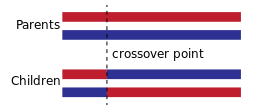
\includegraphics[scale=0.6]{localizacion/screen1.png}
  \caption{Ejemplo de localización de Markov. La gráfica de color rojo representa la distribución de probabilidad. \parencite{Dieter1999}}
  \label{fig:screen1}
\end{figure}


Estudiaremos el ejemplo sencillo que presentan Dieter Fox et. al. para ilustrar los conceptos de la localización de Markov.


Consideremos el entorno mostrado en la figura~\ref{fig:screen1}. Para simplificar, asumamos que el robot sólo puede moverse en una dimensión (enfrente-atrás). Ahora, supongamos que posicionamos el robot en algún lugar aleatorio del entorno, pero no le informamos al robot cuál es su posición. La localización de Markov representa este estado de \quotes{confusión} como una distribución de probabilidad uniforme sobre todo el conjunto de posibles posiciones del entorno, como lo muestra la primer gráfica de la figura~\ref{fig:screen1}. Asumamos que el robot hace una medición con sus sensores y determina que está al lado de una puerta. La localización de Markov modifica la distribución de probabilidad de tal manera que las posiciones que se encuentran a un lado de puertas tengan mayor probabilidad, esto queda ilustrado en la segunda gráfica de la figura~\ref{fig:screen1}. Notemos que la distribución resultante es multimodal(\footnote{Multimodal: Que tiene varios puntos máximos.} ), ya que la información obtenida por los sensores es insuficiente para determinar exactamente la posición del robot. También notemos que las posiciones que no se encuentran a un lado de una puerta aún tienen una probabilidad mayor que cero, esto es porque las mediciones de los sensores contienen ruido. Ahora, supongamos que el robot se mueve un metro hacia el frente. La localización de Markov incorpora este movimiento para que la distribución de probabilidad cambie como se representa en la tercer gráfica de la figura~\ref{fig:screen1}. Finalmente, asumamos que el robot vuelve a tomar una medición con sus sensores. Incorporando esta información a la obtenida anteriormente, vemos cómo la distribución de probabilidad cambia (cuarta gráfica de la figura~\ref{fig:screen1}) para asignar una alta probabilidad a la posición del robot, mientras que todas las demás posiciones tienen una probabilidad casi nula \parencite{Dieter1999}. 

\subsection{Desarrollo}

Tomando como base el modelo de Markov que presentan Dieter Fox et. al., el desarrollo de la práctica se dividirá en dos partes: la simulación del ambiente en donde se encuentra el robot y del robot, y la implementación del modelo en este ambiente.

\subsubsection{Simulación del ambiente y del robot}

\noindent Primero, iniciemos con el contenido y especificación del mundo en el cual se moverá el robot. Este mundo contendrá obstáculos y será rectangular (imagínense un cuarto o una oficina), las paredes serán obstáculos y cualquier otra cosa que se pueda encontrar en un cuarto u oficina normal: sillas, mesas, escritorios, etc. Será representado por una matriz de celdas, donde cada celda será cuadrada, podrá ser obstáculo o no y tendrá la longitud de un lado especificado en \(cm\). En la figura~\ref{fig:mapa} pueden apreciar un ejemplo de cómo se vería el mundo del robot representado gráficamente, donde los cuadros color café son obstáculos, el robot es el círculo verde y se muestra la orientación de este con una línea negra.

El robot podrá ocupar cualquier posición del plano de Processing \footnote{Cabe resaltar que para Processing el eje \(y\) se encuentra invertido, esto es, si aumentan el valor de \(y\) en el código, en la visualización esto se reflejará como si estuvieran caminando hacia abajo. }, no estará necesariamente en el centro de alguna celda. De hecho, se necesitará una función que, dada la posición del robot, nos permita saber dentro de qué celda se encuentra. Esta función nos será útil para la implementación del modelo de Markov discretizado.\par

\begin{figure}
  \centering
  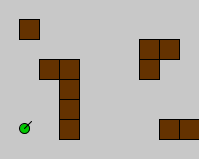
\includegraphics[scale=0.60]{localizacion/mapa.png}
  \caption{Representación visual del ambiente.}
  \label{fig:mapa}
\end{figure}

\paragraph{Movimiento del robot}

\noindent El robot podrá moverse libremente en el ambiente, salvo que se encuentre de frente un obstáculo, o los bordes del mundo ya que son considerados paredes. Este movimiento será controlado por el usuario, ya sea que utilicen las flechas direccionales de su teclado, alguna otra combinación de teclas, botones en la interfaz, o el mecanismo que ustedes prefieran. Lo importante es que el robot pueda moverse en línea recta y girar.\par

El usuario deberá poder especificar qué tanto se moverá el robot al momento de pulsar la tecla o botón requerido, ya sea si se desea cambiar de dirección o moverse en línea recta. Esto será muy importante, ya que necesitan saber la distancia real recorrida y la distancia real de giro para simular las medidas de los sensores.

\paragraph{Simulación de sensores}

\noindent Nuestro robot tendrá tres sensores:

\begin{enumerate}
  \item láser: mide la distancia desde el robot hacia el primer obstáculo en línea recta del sensor. El robot tendrá 8 de estos, ubicados cada \(45\degree\).
  \item odométrico: mide la distancia recorrida por el robot (en cm).
  \item de giro: mide el giro del robot en grados.
\end{enumerate}

Como se darán cuenta más adelante, utilizamos distribuciones Gaussianas para modelar las lecturas de los sensores. Cuando alguien busca armar un robot que tenga sensores, lo primero que debe hacer es calibrarlos para obtener un umbral de error inherente al sensor que se está utilizando para tenerlo en cuenta al momento de programar rutinas o desarrollar el software que permita al robot llegar a su objetivo. Si uno grafica las medidas obtenidas por el sensor versus la medida real, se llega a apreciar que forma una campana centrada en el valor de la medida real ya que los errores pequeños son comunes, pero errores grandes no tanto. Así nosotros podemos suponer que los sensores que estamos modelando generarán mediciones parecidas y utilizamos una distribución de probabilidad normal centrada en el valor real de lo que se mide para obtener la probabilidad de que el robot se encuentre en cierta posición dadas las mediciones recibidas.

\subparagraph{Láser}\medskip
En el caso de este sensor, las mediciones obtenidas pueden cambiar debido a los materiales donde se refleja el láser, entonces utilizaremos ruido gaussiano para simular este error.

Para cada sensor se necesitarán dos parámetros: la media (\( \mu_{laser} \)) y la desviación estándar (\( \sigma_{laser} \)). La desviación estándar es un parámetro que tú debes fijar, éste representa la cantidad de ruido que se introducirá a la medición. Y la media estará dada por la distancia real medida desde el robot hacia el primer obstáculo en línea recta en la dirección del sensor.

Para simular la medición del sensor con ruido, se hará lo siguiente:

\begin{enumerate}
  \item Obtener un número aleatorio utilizando \classname{nextGaussian()} de la clase\\ \classname{java.util.Random}.
  \item Multiplicar el número aleatorio obtenido por la desviación estándar (\( \sigma_{laser} \)).
  \item Sumar a la media (\( \mu_{laser} \)) el resultado anterior.
\end{enumerate}


\subparagraph{Odométrico}\medskip
La manera de simular la medición con ruido de éste sensor es casi idéntica al sensor láser, sólo que en lugar de medir la distancia hacia el obstáculo más cercano usaremos la distancia que el usuario proporcionó para mover al robot. Por ejemplo: Si el usuario decidió mover al robot \(10cm\), la media (\( \mu_{odometrico} \)) sería \(10cm\) y la desviación estándar (\( \sigma_{odometrico} \)) un parámetro especificado por ti.


\subparagraph{De giro}\medskip
Similarmente al sensor odométrico, la media (\( \mu_{de\ giro} \)) sería los grados reales girados y la desviación estándar (\( \sigma_{de\ giro} \)) un parámetro especificado por ti.

\subsubsection{Implementación del modelo de Markov}

\paragraph{Representación interna del mundo}\medskip

El modelo de Markov en el que se basa esta práctica utiliza un modelo del mundo discretizado (como el que usamos para definir área libres y obstáculos). \textit{Dentro de la mente del robot} el mundo será representado por una matriz de tres dimensiones, ya que tenemos tres grados de libertad para el movimiento del robot: \(<x,y,\theta>\), donde \( \theta \) es el ángulo hacia donde está viendo el robot. Estas tres direcciones estarán discretizadas.\par

Recapitulando, en la mente del robot el mundo será representado por un arreglo tridimensional \(<x,y,\theta>\) donde en las coordenadas \(<x,y>\) se tendrá la representación del mundo con celdas, como se especificó al inicio de la sección pasada. Si el robot se encuentra dentro de una celda, \(x\) y \(y\) serán las coordenadas del centro de esta. Y en cuanto al eje \(\theta\), \(\theta\) tomará valores desde 0\degree \ hasta 315\degree, en aumentos de 45\degree. Para cada uno de esos ángulos se tendrá una representación del plano \(<x,y>\) pero con el robot mirando en la dirección discretizada \(\theta\). En la figura~\ref{fig:mapa2} se aprecia un ejemplo de cómo se vería gráficamente la representación del mundo para el robot, con una copia del mundo por cada coordenada \(<x,y,\theta>\). Como puedes ver, la visión del mundo que tiene el robot es mucho más simple de lo que realmente es, y esto puede conducir a que cometa errores.

\begin{figure}
  \centering
  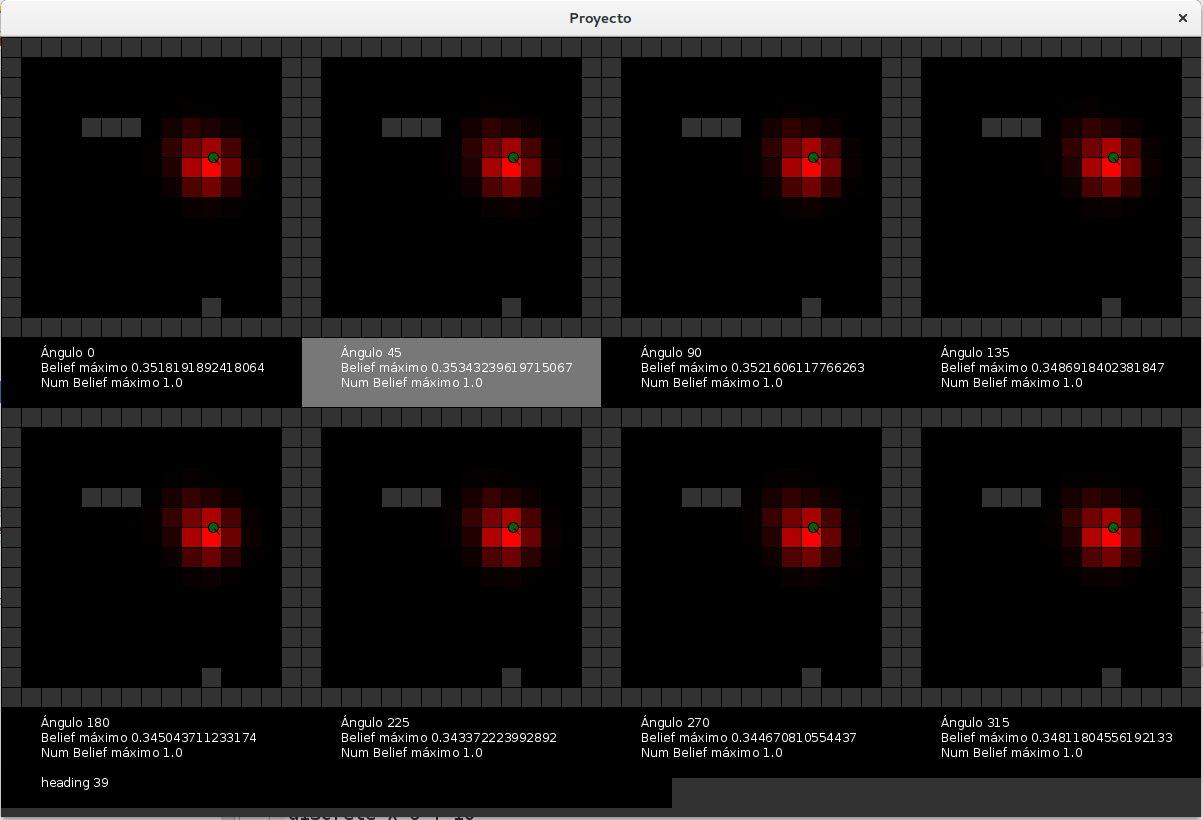
\includegraphics[scale=0.35]{localizacion/mapa_8_dirs.png}
  \caption{Representación del mundo en la mente del robot.}
  \label{fig:mapa2}
\end{figure}

Como habíamos mencionado antes, se necesitará una función que permita obtener la celda en donde se encuentra el robot dadas las coordenadas de éste, pero también se requerirá otra función que nos diga en qué dirección discretizada se encuentra viendo el robot. La función anterior deberá calcular el ángulo al que se encuentra viendo el robot, pero centrado sobre las posibles direcciones de movimiento. Por ejemplo: si el robot se encuentra con una dirección de 12\degree, la función deberá regresar el valor 0\degree, ya que 12\degree \ se encuentra entre (24.5\degree, -24.5\degree].\par

\paragraph{Inicialización}

Deberán posicionar al robot aleatoriamente en el mundo, después deberán calcular la probabilidad de que el robot se encuentre en alguna celda, llamémosle a esta probabilidad \textit{creencia} y representa lo que el robot \textit{cree} acerca de su posición en el mundo \parencite{Dieter1999}. Al inicio esta probabilidad será igual para toda posición porque el robot no sabe dónde está:

\[ P(posici\acute{o}n) = {1 \over \# \ de\ posiciones\ que\ no\ son\ obst\acute{a}culo}\]\medskip

Después, deberán calcular la distancia desde el centro de cada celda al obstáculo más cercano en línea recta, para cada ángulo discretizado. Esta información la deberán guardar para cada posición de tal manera que eviten estar haciendo cálculos cada que sea considerada en el algoritmo siguiente.\footnote{Se sugiere guardar esta información como un atributo de la celda}

\subsection{Notaci\'on}

Definamos la posición discretizada del robot usando una variable tridimensional $l = <x,y,\theta>$, donde $x$ y $y$ son las coordenadas del centro de la celda donde se encuentra el robot y $\theta$ es la dirección discretizada en la que está viendo el robot. A partir de este momento consideraremos únicamente variables discretizadas. Sea $l_t$ la posición real del robot en el tiempo $t$, y $L_t$ la variable aleatoria que modela la probabilidad de que el robot se encuentre en una posición $l$ dada.

Como el robot no sabe su posición exacta, su \textit{creencia} o $Bel(L_t)$ es una distribución de probabilidad \(P(L)\) sobre el espacio de posibles posiciones. Esta \textit{creencia} nos permite saber cuál es la probabilidad de que se encuentre en una celda $l$ en el tiempo $t$, formalmente $Bel(L_t = l)$. Sea \(n\) el número de posiciones posibles.


También aprovecharé para definir a las lecturas de los sensores como: $s_T$ la lectura del láser, $\theta_T$ la lectura del giro y $a_T$ la lectura del sensor odométrico. Sean:

\begin{description}
  \item[$P(s_T \mid l)$] es la probabilidad de que se haya obtenido una medición \(s_T\) si el robot se encuentra en la posición \(l\). Calcularemos esta probabilidad como:
  \begin{align}
    P(s_T \mid l) = {1 \over (\sqrt{2\pi}\sigma_{l\acute{a}ser2})}*\me^{({{-(s_T - \mu_{l\acute{a}ser2})^2} \over {2\sigma_{l\acute{a}ser2}^2}})}
    \label{eq:Pmedicion}
  \end{align}
  donde \(\sigma_{l\acute{a}ser2}\) modela, en parte, el error del sensor y el error por la discretización del mundo, y \(\mu_{l\acute{a}ser2}\) es la distancia desde el centroide de la celda de la posición \(l\) hacia el primer obstáculo.
  \item[$P(\theta \mid \theta', \theta_T)$] es la probabilidad de que el robot esté mirando en el ángulo \(\theta\) de la posición \(l\) dado que se encontraba mirando en el ángulo \(\theta'\) de la posición \(l'\) y se giró un ángulo \(\theta_T\). Supondremos que al girar, el robot no cambia de celda. Calcularemos esta probabilidad como:
  \begin{align}
    P(\theta \mid \theta', \theta_T) = {1 \over (\sqrt{2\pi}\sigma_\theta)}*\me^{({{[\theta_T - (\theta - \theta')]^2} \over {{(\sigma_\theta)}^2}})}
    \label{eq:Podometro}
  \end{align}
  donde \(\sigma_{\theta}\) modela, en parte, el error del sensor y el error por la discretización del mundo. Esta variable será definida por ustedes.
  \item[$P(l \mid l', a_T)$] es la probabilidad de que el robot esté en la posición \(l\) dado que se encontraba en la posición \(l'\) y se avanzó \(a_T\) cms. Calcularemos esta probabilidad como:
  \begin{align}
    P(l \mid l', a_T) = {1 \over (\sqrt{2\pi}\sigma)}*\me^{ -{{1} \over {2}} {{[{ {{ (x' + a_T \cos \theta' - x)^2 } +  { (y' + a_T \sen \theta' - y)^2 } } } + {(\theta' - \theta)^2}]}\over{\sigma^2}}}
    \label{eq:Pgiro}
  \end{align}
  con $\sigma$  modelando el error del sensor.\footnote{Recuerden utilizar radianes, ya que las funciones de \classname{Java} están definidas en radianes.}

\end{description}


Una vez definida la notación, procederemos a ver el algoritmo completo de esta técnica de localización.

 % A estas lecturas se les tendrá que agregar ruido, esto lo lograrán especificando algunas variables:\\

% \begin{enumerate}
%   \item $\sigma$: la varianza de la distribución normal utilizada más adelante.\\
%   \item $S$: porcentaje de ruido de la lectura del odómetro, se usa para calcular $\sigma_x$ y $\sigma_y$.
%   \item $\sigma_\theta$: ruido para la lectura del sensor de giro.
% \end{enumerate}



\subsection{Algoritmo}

\noindent El algoritmo es el siguiente:\medskip

\begin{algorithmic}
  \ForAll{$posicion$ $l$ en $mundo$} \Comment{Inicialización}
    \State $Bel(L_0 = l)\gets P(L_0 = l) = {1 \over n}$
  \EndFor
  \ForAll{$posicion$ $l$ en $mundo$}
    \State $determinar\ las\ distancias\ hacia\ obst\acute{a}culos$
  \EndFor
  \While{$true$}
    \Comment{Se recibió comando o medición del láser}
    \If{no se movió el robot} \Comment{Se recibió medición del láser}
      \State $\alpha_T \gets 0$ \Comment{Constante de normalización}
      \ForAll{$posicion$ $l$ en $mundo$}
        \State $Bel(L_T = l) \gets P(s_T \mid l)*Bel(L_{T-1} = l)$
        \State $\alpha_T \gets \alpha_T + Bel(L_T = l)$
      \EndFor
      \ForAll{$posicion$ $l$ en $mundo$}
      \Comment{Ahora se normaliza la creencia}
        \State $Bel(L_T = l) \gets {\alpha_T}^{-1} * Bel(L_T = l)$
      \EndFor
    \EndIf
    \If{se movió el robot}
      \If{se obtuvo $\theta_T$}
        \Comment{Se obtuvo una lectura del sensor de giro}
        \ForAll{$posicion$ $l$ en $mundo$}
          \State $Bel(L_T = l) \gets [\sum_{\theta'} P(\theta \mid \theta', \theta_T)*Bel(L_{T-1} = l)]$
        \EndFor
      \EndIf
      \If{se obtuvo $a_T$}
        \Comment{Se obtuvo una lectura del sensor odométrico}
        \ForAll{$posicion$ $l$ en $mundo$}
          \State $Bel(L_T = l) \gets [\sum_{l'} P(l \mid l', a_T)*Bel(L_{T-1} = l')]$
        \EndFor
      \EndIf
    \EndIf
  \EndWhile
\end{algorithmic}

\parencite{Dieter1999}

% Si se recibe una lectura del sensor odométrico, por cada celda del mundo, deberán hacer un recorrido por las demás celdas, calculando $\int P(l \mid l', \alpha_T)*Bel(L_T-1 = l')dl$, donde $P(l \mid l', \alpha_T)$ es una variable aleatoria gaussiana tridimensional $G_{x,y,\theta}$ integrada sobre las posiciones de $l$ y $l'$ y desde $\theta + 45\degree/2$ a $\theta - 45\degree/2$.

\subsection{Desarrollo e implementaci\'on}

\subsubsection{Tips}

\begin{itemize}
  \item Tengan bien identificado cuál es su eje X, Y y \(\theta\) en las matrices utilizadas para la simulación.
  \item Utilicen coordenadas polares para todo cálculo, y sólo utilicen grados para visualización, esto les permitirá tener un mayor grado de exactitud y evitan gastar en convertir grados a coordenadas polares en cada operación.
  \item Presten mucha atención en las fórmulas utilizadas, ya que algunas piden sumar la probabilidad sobre un eje, otras piden sumar sobre todas las posiciones del mundo.
  \item Normalicen la creencia cuando el robot gire o se mueva, no solo cuando se reciba una medición del láser. Esto les permitirá compensar errores de redondeo al hacer los cálculos correspondientes.
  \item Hagan una copia del mundo antes de realizar cualquier cálculo, ya que requieren tener la creencia para cada posición en el tiempo \(t-1\) para calcular \(t\). O guarden las creencias recién calculadas en una matriz auxiliar, para luego copiarlas al mundo.
\end{itemize}


\subsection{Requisitos y resultados}

Esto se implementará en processing, recuerden que debe estar bien hecho y comentado, ya que esta práctica vale el 20\% de su calificación. Su aplicación deberá mostrar el mundo, los obstáculos y la probabilidad de cada celda para cada ángulo usando distintos colores o gradientes de un mismo color.

Todo lo anterior lo deberán anexar a la carpeta de la práctica, listo para cargarlo y probarlo. En el \classname{readme} deben especificar cómo se ejecuta, cómo se cargan los archivos, etc. Tampoco olviden comentar su código.
